%!TEX program = xelatex
\documentclass[11pt, aspectratio=169]{beamer}
\usefonttheme{professionalfonts}

\usepackage{amsmath}
\usepackage{fontspec}
\usepackage{graphicx}
\usepackage{import}
\usepackage{kotex}
\PassOptionsToPackage{table}{xcolor}
\usepackage{calc}
\usepackage{listings}
\usepackage{indentfirst}
\usepackage{tabularx}
\usepackage{ulem}
\usepackage{multicol}
\usepackage{epigraph}
\usepackage[many]{tcolorbox}
\usepackage{tabto}   
\usepackage{adjustbox}

\definecolor{boj}{RGB}{0,118,191}
\definecolor{ucpc-orange}{RGB}{255,153,0}
\definecolor{acgreen}{RGB}{0,159,107}
\definecolor{wared}{RGB}{231,76,60}

\definecolor{acbronze}{RGB}{173,86,0}
\definecolor{acsilver}{RGB}{67,95,122}
\definecolor{acgold}{RGB}{236,154,0}
\definecolor{acplatinum}{RGB}{39,226,164}
\definecolor{acdiamond}{RGB}{0,180,252}
\definecolor{acruby}{RGB}{255,0,98}

\setbeamercolor{title}{fg=black}
\setbeamercolor{frametitle}{fg=ucpc-orange}
\setbeamercolor{structure}{fg=ucpc-orange}

\linespread{1.2}
\everymath{\displaystyle}

\graphicspath{ {./images/} }
\lstset{basicstyle=\footnotesize\ttfamily,breaklines=true}

\newcommand{\translation}[1]{\textsuperscript{#1}}

\setlength\fboxsep{0pt}

\newcommand{\complexity}[1]{$\mathcal{O}\left({#1}\right)$}
\newcommand{\difficulty}[1]{\includegraphics[width=1em,natwidth=1000,natheight=1000]{#1.svg.png}}
\newcommand{\norm}[1]{\left\lVert#1\right\rVert}

\usetheme{Ucpc2020}
\usetikzlibrary{arrows.meta,matrix,decorations.pathreplacing}

\title{2024 SCON}
\subtitle{}
\author{Official Solutions}
\date{2024년 5월 11일}

\begin{document}
    \setcounter{framenumber}{-1}
    \frame{\titlepage}

    \begin{frame} %
        \textbf{주최} %
        \begin{itemize}
            \item 숭실대학교 IT대학
        \end{itemize}
        \vspace{3mm}
        \textbf{주관} %
        \begin{itemize}
            \item 컴퓨터학부 문제해결 소모임 SCCC
        \end{itemize}
        \vspace{3mm}
        \textbf{후원} %
        \begin{itemize}
            \item 현대모비스
            \item 퓨리오사AI
            \item Jane Street
            \item 스타트링크
        \end{itemize}
    \end{frame}
    
    \begin{frame}
        \textbf{운영\&출제} %
        \begin{itemize}
            \item 김성주 \tabto{1.5cm} \texttt{rla777} \tabto{8cm} {\color{gray} 숭실대학교 컴퓨터학부}
            \item 나정휘 \tabto{1.5cm} \texttt{jhnah917} \tabto{4cm} {\color{gray} } \tabto{8cm} {\color{gray} 숭실대학교 컴퓨터학부}
            \item 박찬솔 \tabto{1.5cm} \texttt{chansol} \tabto{4cm} {\color{gray} } \tabto{8cm} {\color{gray} 숭실대학교 컴퓨터학부}
            \item 유상원 \tabto{1.5cm} \texttt{sangwon090} \tabto{4cm} {\color{gray} } \tabto{8cm} {\color{gray} 숭실대학교 컴퓨터학부}
            \item 오주원 \tabto{1.5cm} \texttt{kyo20111} \tabto{4cm} {\color{gray} } \tabto{8cm} {\color{gray} 숭실대학교 소프트웨어학부}
            \item 진세림 \tabto{1.5cm} \texttt{qwerty1120} \tabto{8cm} {\color{gray} 숭실대학교 컴퓨터학부}
        \end{itemize}
        \vspace{3mm}
    \end{frame}

    \begin{frame}%
        \textbf{검수} %
        \begin{itemize}
            \item 김영현 \tabto{1.5cm} \texttt{kipa00} \tabto{8cm} {\color{gray} 서울대학교 컴퓨터공학부}
            \item 윤교준 \tabto{1.5cm} \texttt{yclock} \tabto{8cm} {\color{gray} 서울대학교 컴퓨터공학부}
            \item \adjustbox{scale={.66}{1}}{白崎杏子} \tabto{1.5cm} \texttt{cologne } \tabto{4cm} {\color{gray} } \tabto{8cm} {\color{gray} 開拓団訓練所}
        \end{itemize}
        \vspace{3mm}
        \textbf{테스트} %
        \begin{itemize}
            \item 우민규 \tabto{1.5cm} \texttt{mingyu331} \tabto{8cm} {\color{gray} 서울과학고등학교}
            \item 이지언 \tabto{1.5cm} \texttt{ez\_code} \tabto{8cm} {\color{gray} 연세대학교 아시아학과}
            \item 진민성 \tabto{1.5cm} \texttt{m4ushold} \tabto{8cm} {\color{gray} 숭실대학교 소프트웨어학부}
        \end{itemize}
    \end{frame}

    \begin{frame}%
        \textbf{포스터, 명찰, 상장 디자인} %
        \begin{itemize}
            \item 박수현 \tabto{1.5cm} \texttt{shiftpsh} \tabto{8cm} {\color{gray} 서강대학교 컴퓨터공학과}
        \end{itemize}
        \vspace{3mm}
        \textbf{문제지, 풀이 슬라이드 제작} %
        \begin{itemize}
            \item 김영현 \tabto{1.5cm} \texttt{kipa00} \tabto{8cm} {\color{gray} 서울대학교 컴퓨터공학부}
            \item 나정휘 \tabto{1.5cm} \texttt{jhnah917} \tabto{4cm} {\color{gray} } \tabto{8cm} {\color{gray} 숭실대학교 컴퓨터학부}
            \item 박수현 \tabto{1.5cm} \texttt{shiftpsh} \tabto{8cm} {\color{gray} 서강대학교 컴퓨터공학과}
        \end{itemize}
    \end{frame}
    
    \begin{frame}%
        \textbf{대회 현장 스태프} %
        \begin{itemize}
            \item 길수민 \tabto{1.5cm} \texttt{2093ab} \tabto{8cm} {\color{gray} 숙명여자대학교 소프트웨어학부}
            \item 김영현 \tabto{1.5cm} \texttt{kipa00} \tabto{8cm} {\color{gray} 서울대학교 컴퓨터공학부}
            \item 박경욱 \tabto{1.5cm} \texttt{sk091204091204} \tabto{8cm} {\color{gray} 연세대학교 인공지능학과}
            \item 우민규 \tabto{1.5cm} \texttt{mingyu331} \tabto{8cm} {\color{gray} 서울과학고등학교}
            \item 이지언 \tabto{1.5cm} \texttt{ez\_code} \tabto{8cm} {\color{gray} 연세대학교 아시아학과}
            \item 정은채 \tabto{1.5cm} \texttt{celina324} \tabto{8cm} {\color{gray} 이화여자대학교 컴퓨터공학과}
            \item 조다니엘 \tabto{1.5cm} \texttt{arduinocc04} \tabto{8cm} {\color{gray} 서강대학교 컴퓨터공학과}
            \item 진민성 \tabto{1.5cm} \texttt{m4ushold} \tabto{8cm} {\color{gray} 숭실대학교 소프트웨어학부}
            \item 천민재 \tabto{1.5cm} \texttt{open\_mind} \tabto{8cm} {\color{gray} 홍익대학교 캠퍼스자율전공(서울)}
            \item 운영\&출제진 모두
        \end{itemize}
    \end{frame}
    
    \begin{frame}{\textbf{Sponsors}}
        \begin{center}
            
\includegraphics[width=0.36\linewidth]{images/logos/mobis.jpg}\\
            \vspace{10mm}
            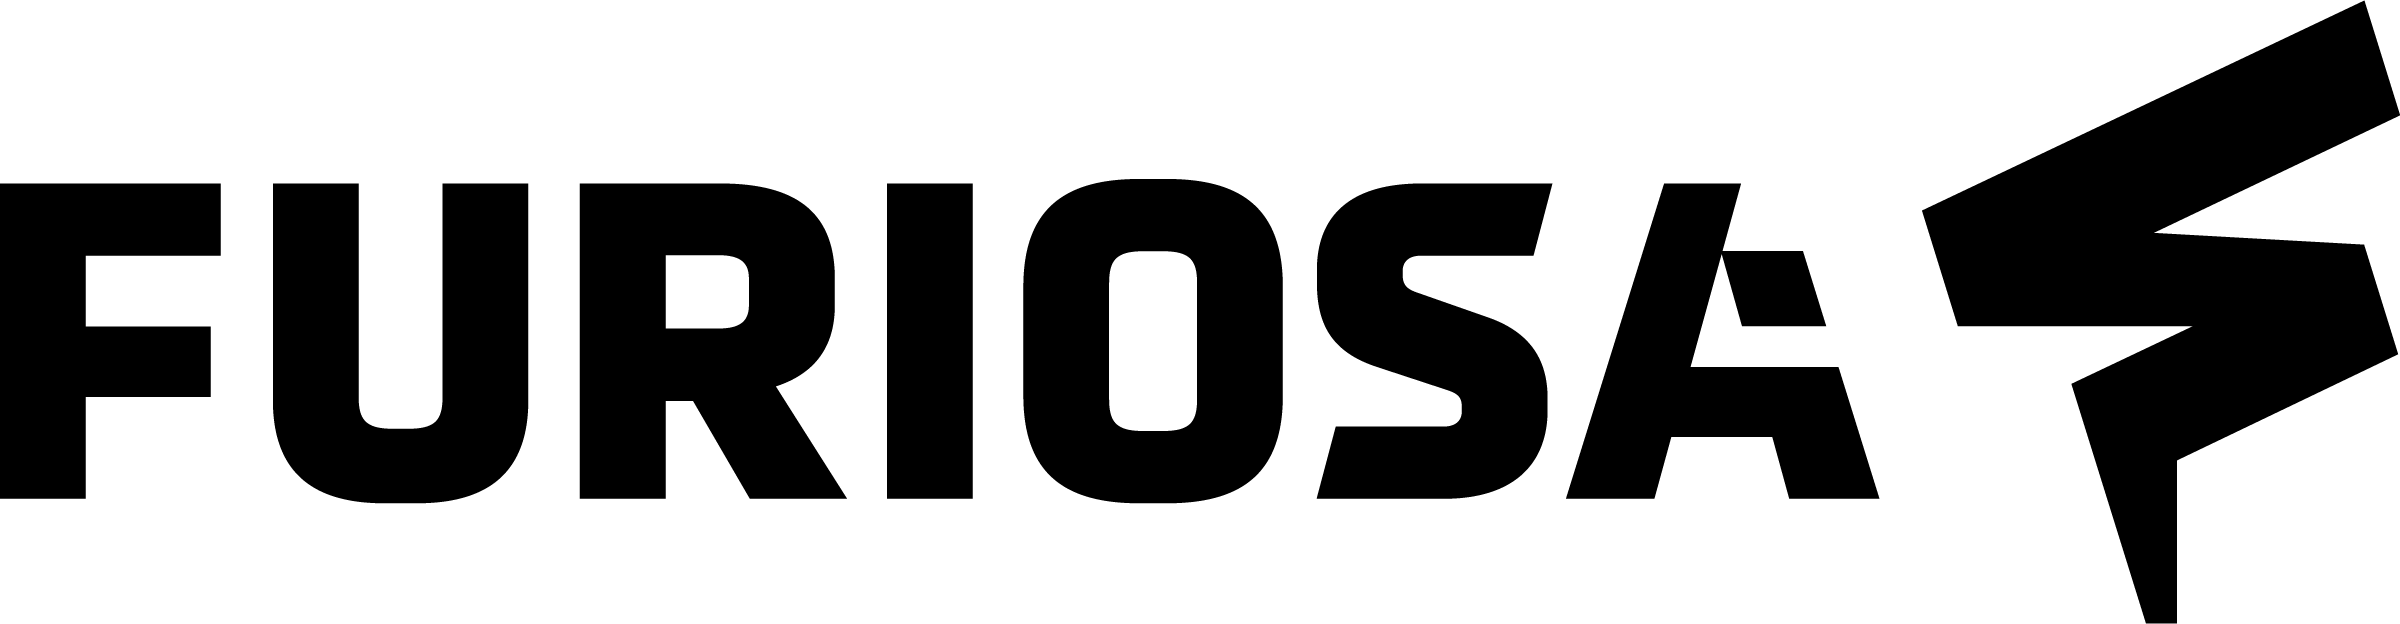
\includegraphics[width=0.36\linewidth]{images/logos/Furiosa_AI.png}
        \end{center}
    \end{frame}

    \begin{frame}{\textbf{Sponsors}}
        \begin{center}
            
\includegraphics[width=0.36\linewidth]{images/logos/JaneStreet.png}\\
            \vspace{10mm}
            
\includegraphics[width=0.36\linewidth]{images/logos/startlink.png}
        \end{center}
    \end{frame}
    
    \begin{frame} % No title at first slide
        \begin{center}
            \begin{tabular}{cl|l|l}
                \hline
                문제 & & 의도한 난이도 & 출제자 \\
                \hline
                \hline
                \textbf{A} & 과민성 대장 증후군 & \textbf{\color{acbronze} Easy} & 유상원 \\
                \textbf{B} & 팀명 정하기 2 & \textbf{\color{acbronze} Easy} & 나정휘 \\
                \textbf{C} & 온데간데없을뿐더러 & \textbf{\color{acbronze} Easy} & 나정휘 \\
                \textbf{D} & 미로 탈출 & \textbf{\color{acsilver} Medium} & 오주원 \\
                \textbf{E} & 수식 고치기 & \textbf{\color{acsilver} Medium} & 박찬솔 \\
                \textbf{F} & 피보나치 기념품 & \textbf{\color{acsilver} Medium} & 나정휘 \\
                \textbf{G} & 시간표 만들기 & \textbf{\color{acgold} Hard} & 박찬솔 \\
                \textbf{H} & 아이템 2 & \textbf{\color{acgold} Hard} & 오주원 \\
                \textbf{I} & 불꽃놀이의 아름다움 & \textbf{\color{acgold} Hard} & 박찬솔 \\
                \textbf{J} & Traveling SCCC President 2 & \textbf{\color{acgold} Hard} & 오주원 \\
                % \textbf{G} & 인공 신경망 (예시) & \textbf{\color{acgold} Hard} & 나정휘 \\ % 핸들 넣을 거면 \texttt{jhnah917}
                % \textbf{X} & 적당히 긴 이름이 필요한데 뭐라고 & \textbf{\color{acplatinum} Challenging} & 박찬솔 \\
                \hline
            \end{tabular}
        \end{center}
    \end{frame}

    \import{solutions/}{2024/irritable-bowel-syndrome.tex}
    \import{solutions/}{2024/team-name-2.tex}
    \import{solutions/}{2024/concat.tex}
    \import{solutions/}{2024/visit-all.tex}
    \import{solutions/}{2024/modify-expression.tex}
    \import{solutions/}{2024/fibonacci-partition.tex}
    \import{solutions/}{2024/create-timetable.tex}
    \import{solutions/}{2024/fork.tex}
    \import{solutions/}{2024/beautiful-fireworks.tex}
    \import{solutions/}{2024/or-path.tex}
    
    \begin{frame} % No title
        \begin{itemize}
            \item 대회 문제의 모범 코드는 https://sccc.kr/scon/2024 에서 확인할 수 있습니다.
            \item 감사합니다.
        \end{itemize}
    \end{frame}
\end{document}
